\begin{figure}[ht]
    \centering
    % 裁剪图片边缘可能存在的白色区域（根据实际情况调整参数）
        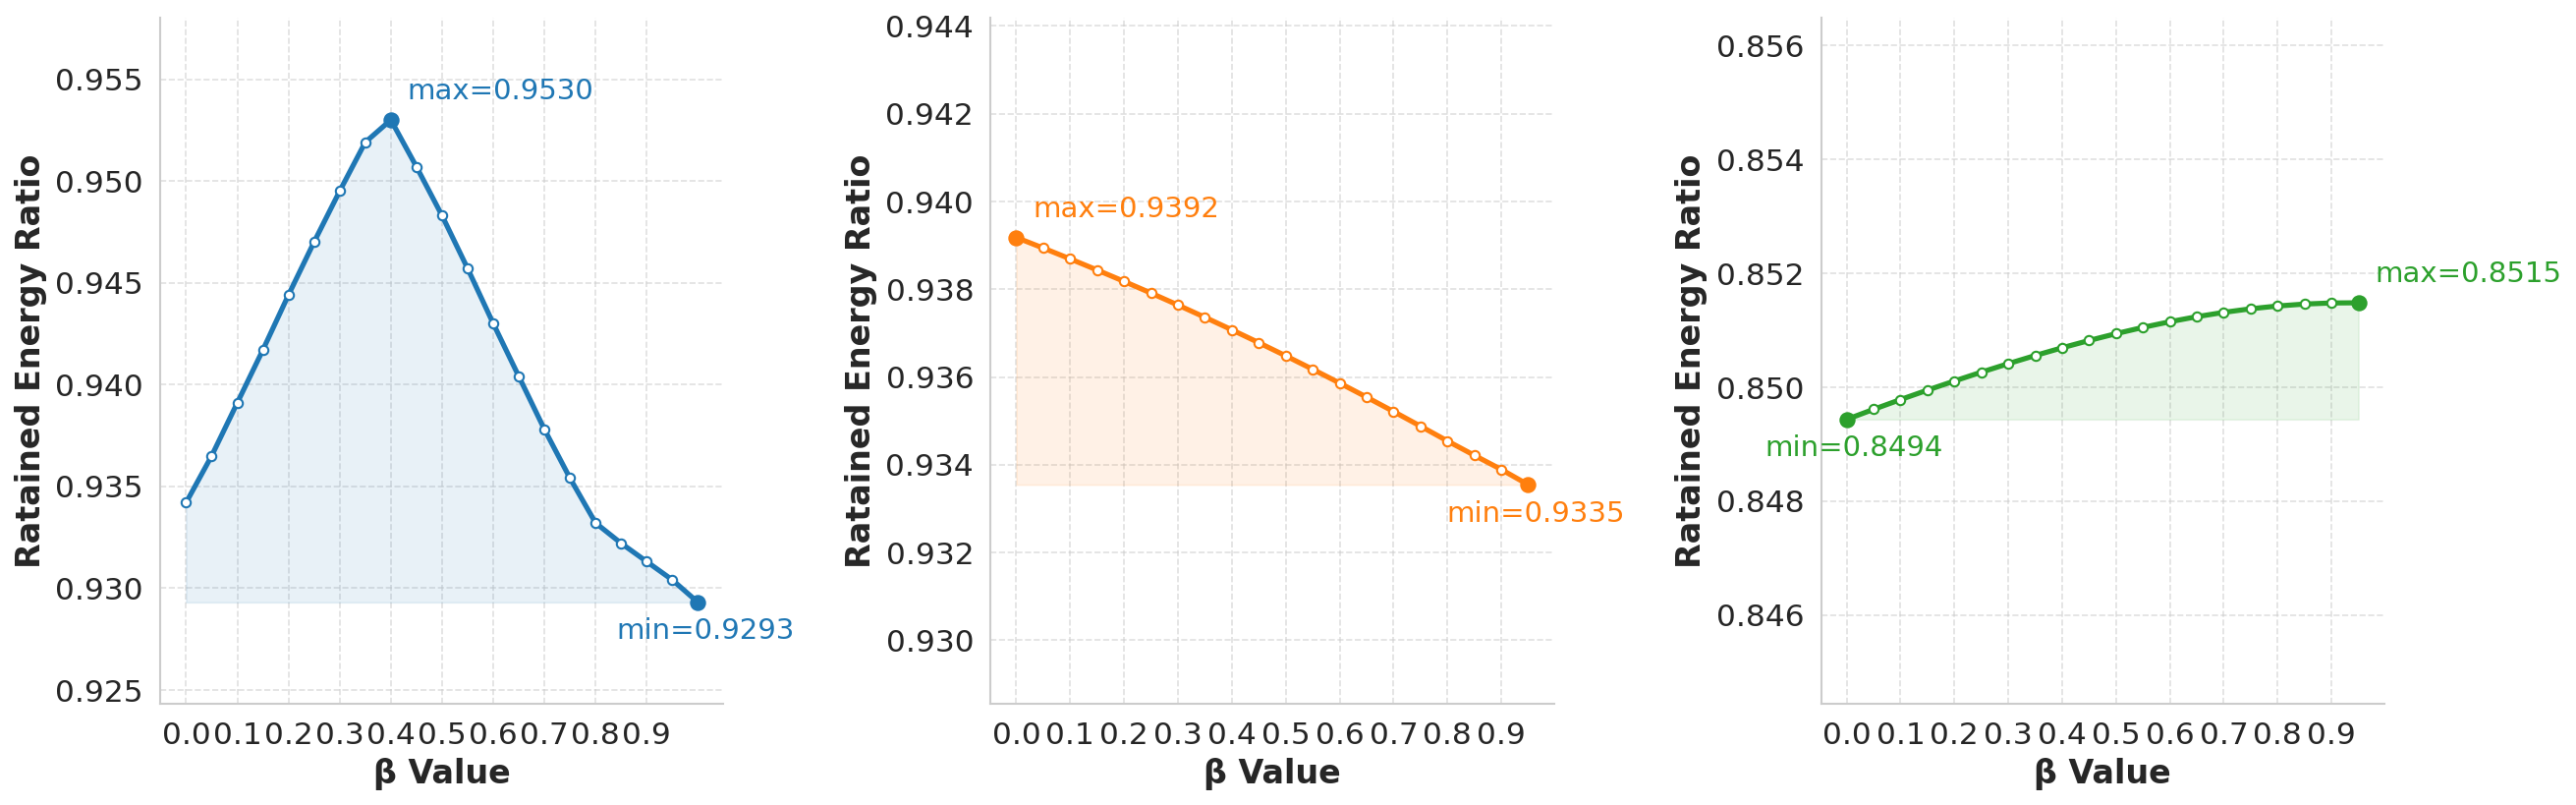
\includegraphics[width=1\linewidth]{figs/three_ratio_of_differnet_beta.png}
    % 调整标题与图片的距离
    \caption{ Using different beta coefficients for the k-proj of LLama3-8B at layer 14, layer 3 and layer 20 after the SVD in Equation~\ref{eq:final svd}, the proportion of retained energy at rank-1228.}
    \label{fig:different beta ratio}  % 标签使用冒号分隔符，符合LaTeX规范
    % 调整图与下文的距离
    \end{figure}